\chapter[Introduction]{Introduction}
\label{sec:introduction}

% \mylabel{%
%
\begin{rotate}{270}
\begin{minipage}{4cm}
\centering\nameref{sec:introduction}
\end{minipage}
\end{rotate}
%
\vspace{4.3cm}\hrule
%
\begin{rotate}{270}
\begin{minipage}{4cm}
\centering\nameref{sec:bg}
\end{minipage}
\end{rotate}
%
\vspace{4.3cm}\hrule
%
\begin{rotate}{270}
\begin{minipage}{4cm}
\centering\nameref{chp:mpi_for_the_r_user}
\end{minipage}
\end{rotate}
%
\vspace{4.3cm}\hrule
%
\begin{rotate}{270}
\begin{minipage}{4cm}
\centering\nameref{sec:statistics_examples}
\end{minipage}
\end{rotate}
%
\vspace{4.3cm}\hrule
}%


% chap:dmat
% chap:makedmat
% chap:basicdmat
% cpht:avdstat
% sec:reader
% chp:pbdNCDF4

\inspire%
{There are things which seem incredible to most men who have not studied Mathematics.}%
{Archimedes of Syracus}



\section{What is pbdR?}
The ``Programming with Big Data in R'' project~\citep{pbdR2012}
(\pbdR for short) is a project that aims to elevate the statistical programming
language \proglang{R}~\citep{Rcore} to leadership-class computing platforms.
The main goal is empower data scientists by bringing flexibility and a big
analytics toolbox to big data challenges, with an emphasis on productivity,
portability, and performance.  We achieve this in part by mapping high-level
programming syntax to portable, high-performance, scalable, parallel libraries.
In short, we make \proglang{R} scalable.

\begin{figure}[h]
 \centering
 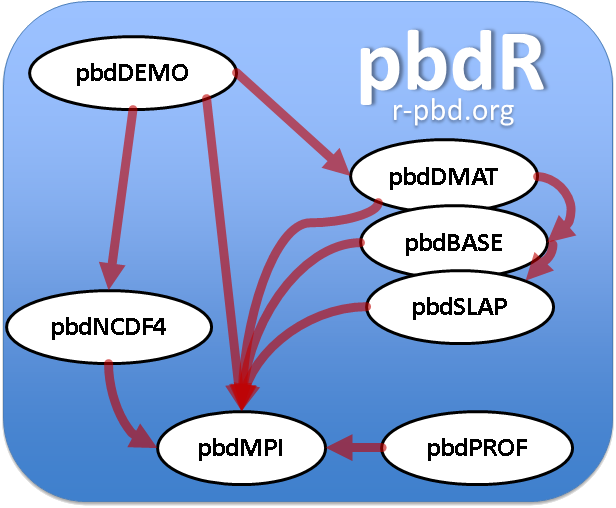
\includegraphics[scale=.65]{pbdDEMO-include/pics/pbdR.png}
 \caption{pbdR Packages}
 \label{fig:pbdrpackages}
\end{figure}

Figure~\ref{fig:pbdrpackages} shows the current list of \pbdR
packages released
to the CRAN (\url{http://cran.r-project.org}), and how they depend on each
other. More explicitly, the current \pbdR packages
\citep{Chen2012pbdMPIpackage,Chen2012pbdSLAPpackage,Schmidt2012pbdBASEpackage,
Schmidt2012pbdDMATpackage,Patel2013pbdNCDF4package,Schmidt2013pbdDEMOpackage}
are:

\begin{itemize}
 \item \pkg{pbdMPI} --- an efficient interface to MPI~\citep{MPI1994} with a
       focus on Single Program/Multiple Data (SPMD)\index{Parallelism!SPMD}
       parallel programming style.
 \item \pkg{pbdSLAP} --- bundles scalable dense linear algebra libraries in
       double precision for \proglang{R}, based on ScaLAPACK
       version 2.0.2~\citep{slug}.~\index{Library!ScaLAPACK}
 \item \pkg{pbdNCDF4} --- Interface to Parallel Unidata
       NetCDF4\index{Library!NetCDF4} format data files~\citep{netcdf}.
 \item \pkg{pbdBASE} --- low-level ScaLAPACK codes and wrappers.
 \item \pkg{pbdDMAT} --- distributed matrix classes and computational methods,
       with a focus on linear algebra and statistics.
 \item \pkg{pbdDEMO} --- set of package demonstrations and examples, and this
       unifying vignette.
\end{itemize}

To try to make this landscape a bit more clear, one could divide
\pbdR packages into those meant for users, developers, or
something in-between.  
\begin{figure}[h]
 \centering
 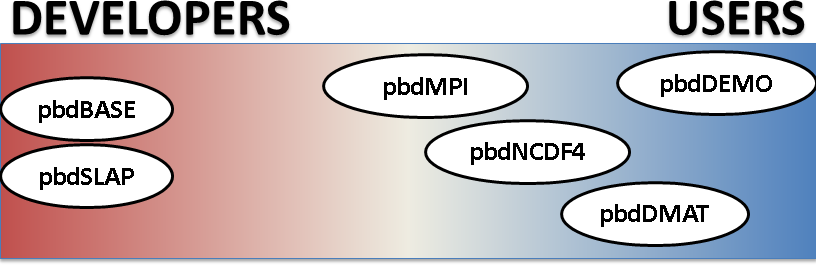
\includegraphics[scale=.55]{pbdDEMO-include/pics/pbdR-packages.png}
 \caption{pbdR Package Use}
 \label{fig:pbdrpackages2}
\end{figure}
Figure~\ref{fig:pbdrpackages2} shows a gradient scale representation, where
more red means the package is more for developers, while more blue means the
package is more for users.  For example, \pkg{pbdDEMO} is squarely meant for
users of \pbdR packages, while \pkg{pbdBASE} and \pkg{pbdSLAP} are
really not meant for general use. The other packages fall somewhere
in-between, having plenty of utility for both camps.

Finally, 
\begin{figure}[h]
 \centering
 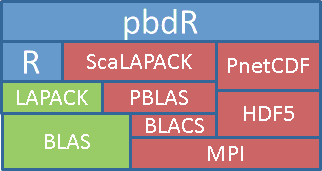
\includegraphics[scale=.85]{pbdDEMO-include/pics/libs.png}
 \caption{pbdR Interface to Foreign Libraries}
 \label{fig:pbdrlibs}
\end{figure}
Figure~\ref{fig:pbdrlibs} shows \pbdR relationship to
high-performance libraries.

In this vignette, we offer many examples using the above \pbdR
packages. Many of the examples are high-level applications and may be commonly
found in basic Statistics. The purpose is to show how to reuse the
preexisting functions and utilities of \pbdR to create minor
extensions which can quickly solve problems in an efficient way.
The reader is encouraged to reuse and re-purpose these functions.

The \pkg{pbdDEMO} package consists of two main parts. The first is a
collection of roughly 20+ package demos. These offer example uses of
the various \pbdR packages. The second is this vignette, which
attempts to offer detailed explanations for the demos, as well as sometimes
providing some mathematical or statistical insight. A list of all of the
package demos can be found in Section~\ref{sec:demolist}.



\section{Why Parallelism?  Why pbdR?}

It is common, in a document such as this, to justify the need for parallelism.
Generally this process goes:

\begin{quote}
\emph{
Blah blah blah Moore's Law, blah blah Big Data, blah blah blah Concurrency.
}
\end{quote}

How about this? Parallelism is cool. Any boring nerd can use one computer,
but using 10,000 at once is another story. We don't call them
\emph{\textbf{supercomputers}} for nothing.

But unfortunately, lots of people who would otherwise be thrilled to do all
kinds of cool stuff with massive behemoths of computation~--- computers with
names like \textbf{KRAKEN}\footnote{
\url{http://www.nics.tennessee.edu/computing-resources/kraken}
} and \textbf{TITAN}\footnote{
\url{http://www.olcf.ornl.gov/titan/}
}~--- are burdened by an
unfortunate reality:  it's really, really hard.
Enter \pbdR. Through our project, we put a shiny new set of
clothes on high-powered compiled code, making massive-scale computation
accessible to a wider audience of data scientists than ever before.
Analytics in supercomputing shouldn't just be for the elites.



\section[Installation]{Installation}
\label{sec:installation}

One can download \pkg{pbdDEMO} from CRAN at
\url{http://cran.r-project.org}, and
the installation can be done with the following commands
\begin{lstlisting}
tar zxvf pbdDEMO_0.2-0.tar.gz
R CMD INSTALL pbdDEMO
\end{lstlisting}
Since \pkg{pbdEMO} depends on other \pbdR packages, please read
the corresponding vignettes if installation of any of them is unsuccessful.





\section{Structure of pbdDEMO}

The \pkg{pbdDEMO} package consists of several key components:

\begin{enumerate}
  \item This vignette
  \item A set of demos in the \code{demo/} tree
  \item A set of benchmark codes in the \code{Benchmarks/} tree
\end{enumerate}

The following subsections elaborate on the contents of the latter two.


\subsection{List of Demos}
\label{sec:demolist}

A full list of demos contained in the \pkg{pbdDEMO} package is provided below.
We may or may not describe all of the demos in this vignette.

\begin{lstlisting}[title=List of Demos]
### (Use Rscript.exe for windows systems)

		      # --------------------- #
		      # II Direct MPI Methods #
		      # --------------------- #

### Chapter 4
# Monte carlo simulation
mpiexec -np 4 Rscript -e "demo(monte_carlo, package='pbdDMAT', ask=F, echo=F)"
# Sample mean and variance
mpiexec -np 4 Rscript -e "demo(sample_stat, package='pbdDMAT', ask=F, echo=F)"
# Binning
mpiexec -np 4 Rscript -e "demo(binning, package='pbdDMAT', ask=F, echo=F)"
# Quantile
mpiexec -np 4 Rscript -e "demo(quantile, package='pbdDMAT', ask=F, echo=F)"
# OLS
mpiexec -np 4 Rscript -e "demo(ols, package='pbdDMAT', ask=F, echo=F)"
# Distributed Logic
mpiexec -np 4 Rscript -e "demo(comparators, package='pbdDMAT', ask=F, echo=F)"

		  # ------------------------------ #
		  # III Distributed Matrix Methods #
		  # ------------------------------ #

### Chapter 6
# Random matrix generation
mpiexec -np 4 Rscript -e "demo(randmat_global, package='pbdDMAT', ask=F, echo=F)"
mpiexec -np 4 Rscript -e "demo(randmat_local, package='pbdDMAT', ask=F, echo=F)"

### Chapter 8
# Sample statistics revisited
mpiexec -np 4 Rscript -e "demo(sample_stat_dmat, package='pbdDMAT', ask=F, echo=F)"
# Verify solving Ax=b at scale
mpiexec -np 4 Rscript -e "demo(verify, package='pbdDMAT', ask=F, echo=F)"
# PCA compression
mpiexec -np 4 Rscript -e "demo(pca, package='pbdDMAT', ask=F, echo=F)"
# OLS and predictions
mpiexec -np 4 Rscript -e "demo(ols_dmat, package='pbdDMAT', ask=F, echo=F)"

		  # ---------------------------- #
		  # IV Reading and Managing Data #
		  # ---------------------------- #

### Chapter 9
# Reading csv
mpiexec -np 4 Rscript -e "demo(read_csv, package='pbdDMAT', ask=F, echo=F)"
# Reading sql
mpiexec -np 4 Rscript -e "demo(read_sql, package='pbdDMAT', ask=F, echo=F)"

### Chapter 10
# Reading and writing parallel NetCDF4
Rscript -e "demo(trefht, package="pbdDEMO", ask = F, echo = F)"
mpiexec -np 4 Rscript -e "demo(nc4_serial, package='pbdDEMO', ask=F, echo=F)"
mpiexec -np 4 Rscript -e "demo(nc4_parallel, package='pbdDEMO', ask=F, echo=F)"
mpiexec -np 4 Rscript -e "demo(nc4_dmat, package='pbdDEMO', ask=F, echo=F)"
mpiexec -np 4 Rscript -e "demo(nc4_gbdc, package='pbdDEMO', ask=F, echo=F)"

### Chapter 11
# Loand/unload balance
mpiexec -np 4 Rscript -e "demo(balance, package='pbdDMAT', ask=F, echo=F)"
# GBD to DMAT
mpiexec -np 4 Rscript -e "demo(gbd_dmat, package='pbdDMAT', ask=F, echo=F)"
# Distributed matrix redistributions
mpiexec -np 4 Rscript -e "demo(reblock, package='pbdDMAT', ask=F, echo=F)"

		  # ---------------------------- #
		  # V Applications               #
		  # ---------------------------- #

### Chapter 13
# Parallel Model-Based Clustering
Rscript -e "demo(iris_overlap, package='pbdDEMO', ask=F, echo=F)"
Rscript -e "demo(iris_serial, package='pbdDEMO', ask=F, echo=F)"
Rscript -e "demo(iris_gbd, package='pbdDEMO', ask=F, echo=F)"
Rscript -e "demo(iris_dmat, package='pbdDEMO', ask=F, echo=F)"

### Chapter 14
mpiexec -np 4 Rscript -e "demo(task_pull, package='pbdMPI', ask=F, echo=F)"
mpiexec -np 4 Rscript -e "demo(phyclust_bootstrap, package='pbdDEMO', ask=F, echo=F)"

### Chapter 15
mpiexec -np 4 Rscript -e "demo(mcmc_galaxy, package='pbdDEMO', ask=F, echo=F)"
\end{lstlisting}





\subsection{List of Benchmarks}

At the time of writing, there are benchmarks for computing covariance, linear
models, and principal components. The benchmarks come in two variants. The
first is an ordinary set of benchmark codes, which generate data of specified
dimension(s) and time the indicated computation. This operation is replicated
for a user-specified number of times (default 10), and then the timing results
are printed to the terminal.  

From the \code{Benchmarks/} subtree, the user can run the first set of
benchmarks with, for example, 4 processors by issuing any of the commands:
\begin{lstlisting}
### (Use Rscript.exe for windows systems)
mpiexec -np 4 Rscript cov.r
mpiexec -np 4 Rscript lmfit.r
mpiexec -np 4 Rscript pca.r
\end{lstlisting}

The second set of benchmarks are those that try to find the ``balancing''
point where, for the indicted computation with user specified number of
cores, the computation is performed faster using \pbdR
than using serial \proglang{R}. In general, throwing a bunch of cores at
a problem may not be the best course of action, because parallel algorithms
(almost always) have inherent overhead over their serial counterparts that
can make their use ill-advised for small problems. But for sufficiently
big (which is usually not very big at all) problems, that overhead should
quickly be dwarfed by the increased scalability.

From the \code{Benchmarks/} subtree, the user can run the second set of
benchmarks with, for example, 4 processors by issuing any of the commands:
\begin{lstlisting}
### (Use Rscript.exe for windows systems)
mpiexec -np 4 Rscript balance_cov.r
mpiexec -np 4 Rscript balance_lmfit.r
mpiexec -np 4 Rscript balance_pca.r
\end{lstlisting}

Now we must note that there are other costs than just statistical
computation. There is of course the cost of disk IO (when dealing with real
data). However, a parallel file system should help with this, and for large
datasets should actually be faster anyway. The main cost not measured here
is the cost of starting all of the R processes and loading packages.
Assuming \proglang{R} is not compiled statically (and it almost certainly
is not), then this cost is non-trivial and somewhat unique to very large
scale computing. For instance, it took us well over an hour to start
12,000 \proglang{R} sessions and load the required packages on the
supercomputer
KRAKEN\footnote{See \url{https://en.wikipedia.org/wiki/Kraken_(supercomputer)}}.  This problem is not unique to \proglang{R}, however.  It affects any project that has a great deal of dynamic library loading to do.  This includes \proglang{Python}, although their community has made some impressive strides in dealing with this problem.




\section{Exercises}
\label{sec:introduction_exercise}

\begin{enumerate}[label=\thechapter-\arabic*]
\item
Read the MPI wikipedia page \url{https://en.wikipedia.org/wiki/Message_Passing_Interface}
including it's history, overview, functionality, and concepts sections.

\item
Read the \pkg{pbdMPI} vignette and install either
OpenMPI~\index{Library!OpenMPI} (\url{http://www.open-mpi.org/}) or
MPICH2~\index{Library!MPICH2}
(\url{http://www.mcs.anl.gov/research/projects/mpich2/}),
 and test if the installation is correct (see \url{http://www.r-pbd.org/install.html} for more details).
\label{ex:introduction2}

\item
After completing Exercise~\ref{ex:introduction2},
install all \pbdR packages and run each package's demo codes.
\end{enumerate}

